\begin{center}
\begin{tikzpicture}[node distance =  2.75cm,auto,fontscale=0.01,x=1cm,y=1cm]

 \visible<1-15>{\node [rectangle,minimum width=8cm,minimum height =8cm,anchor=center, 
 	path picture= {\node at (path picture bounding box.center){\includegraphics[width=8cm]{figures/dim_error}{}};}](ff) at (0,1){};}
% 	\draw[help lines,xstep=1,ystep=1] (-3,-2) grid (4,5);
 %	 	\draw[help lines,xstep=0.5,ystep=0.5,thin,gray] (-3,-2) grid (4,5);
% 	\foreach \x in {-5,-4,...,5} { \node [anchor=north] at (\x,0) {\x}; }
 %	\foreach \y in {-5,-4,...,5} { \node [anchor=east] at (0,\y) {\y}; }


 \visible<1-2>{\node[rectangle,minimum width=1.5cm,fill=white,minimum height=0.5cm,opacity=1,rounded corners] (RAC155C) at (2.85,-0.57){};}
 \visible<1>{\node[rectangle,minimum width=1.5cm,fill=white,minimum height=0.5cm,opacity=1,rounded corners] (MCDLC) at (-2.15,3.63){};} 
\visible<1->{\node at (0,-2.55) {\begin{footnotesize}Janet, J.P., and Kulik, H.J. \textit{J. Phys. Chem. A}, 2017,121, 46, 8939-8954.\end{footnotesize}};}

\visible<1-13>{\node[rectangle,minimum width=1.5cm,fill=white,minimum height=0.5cm,opacity=1,rounded corners] (LS28) at (-2.0,-0.85){};}
\visible<1-14>{\node[rectangle,minimum width=1.5cm,fill=white,minimum height=0.5cm,opacity=1,rounded corners] (rF41C) at (-1.58,-0.45){};}

  \visible<1-5>{\node[ rectangle,minimum width=1.5cm,fill=white,minimum height=0.5cm,opacity=1,rounded corners] (UVC) at (0.20,-0.64){};}
 \visible<1-9>{\node[rectangle,minimum width=1.5cm,fill=white,minimum height=0.5cm,opacity=1,rounded corners] (RFE43C) at (-1.5,0.85){};} 
 
 
%%% UV
\visible<4-6>{\node [rectangle,anchor=center, ,minimum width=3cm,minimum height =2cm,ultra thick, blue,draw,
	path picture= {\node at (path picture bounding box.center){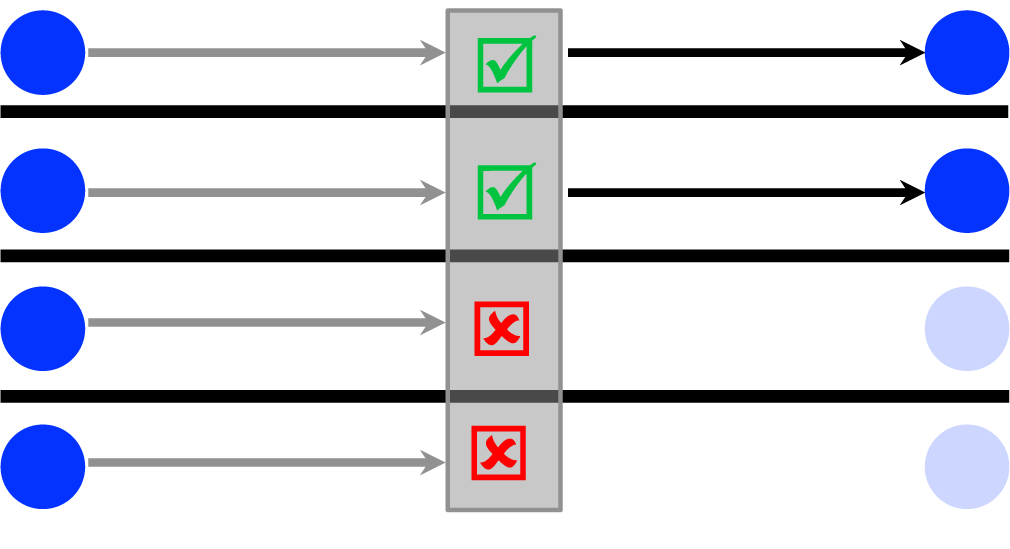
\includegraphics[width=3cm]{images/uv}{}};}](uvf) at (1.25,1.5){};}                
\visible<5-6>{\path[draw,ultra thick,blue] (RAC155C.north) edge[bend right]  (uvf.south){};}
\visible<6>{\path[draw,ultra thick,blue] (uvf.south) edge[bend right,->]  (UVC.north){};}



%%% RFE
\visible<8-10>{\node [rectangle,anchor=center, ,minimum width=3cm,minimum height =2cm,ultra thick, blue,draw,
	path picture= {\node at (path picture bounding box.center){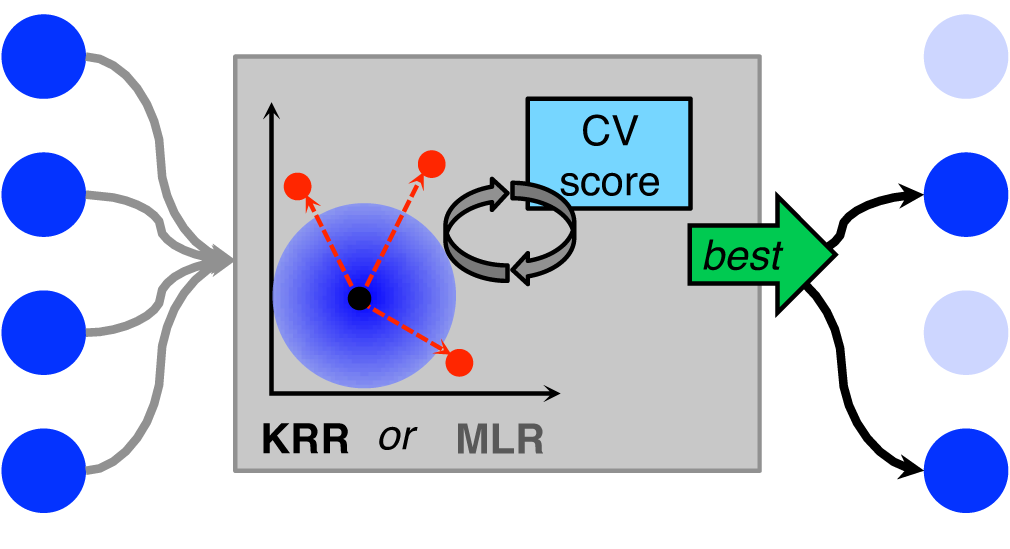
\includegraphics[width=3cm]{images/wrap}{}};}](rfe) at (0.5,3){};}                
\visible<9-10>{\path[draw,ultra thick,blue] (RAC155C.north) edge[bend right]  (rfe.south){};}
\visible<10>{\path[draw,ultra thick,blue] (rfe.south) edge[bend right,->]  (RFE43C.north){};}

 
 
%%% em
\visible<12-15>{\node [rectangle,anchor=center, ,minimum width=3cm,minimum height =2cm,ultra thick, blue,draw,
	path picture= {\node at (path picture bounding box.center){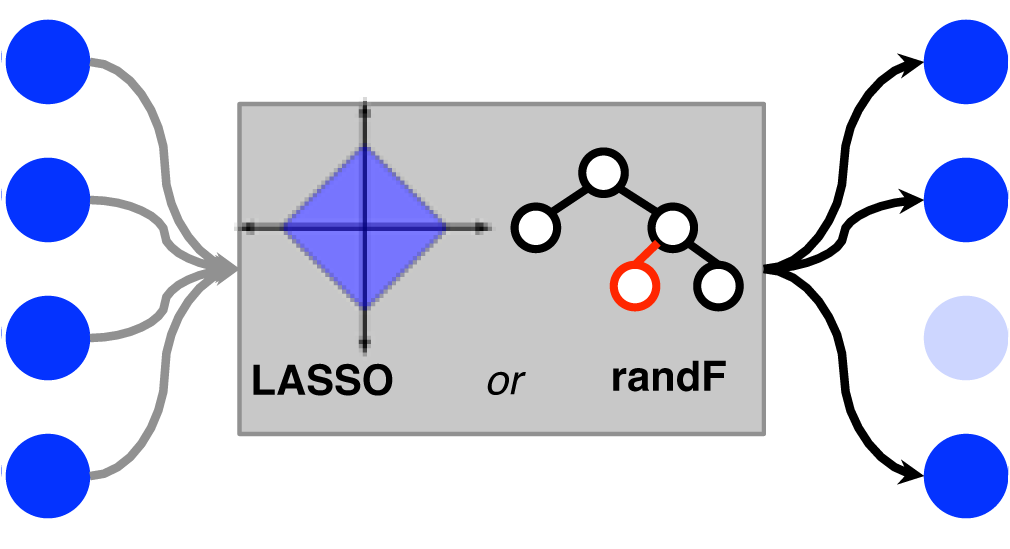
\includegraphics[width=3cm]{images/em}{}};}](em) at (0.5,2.30){};}                
\visible<13-15>{\path[draw,ultra thick,blue] (RAC155C.north) edge[bend right]  (em.south){};}

 \visible<15>{\path[draw,ultra thick,blue] (em.south) edge[bend right,->]  (rF41C.north){};}
\visible<14>{\path[draw,ultra thick,blue] (em.south) edge[bend right,->]  (LS28.north){};}

\end{tikzpicture}
\end{center}